

\begin{figure}[!h]
\centering
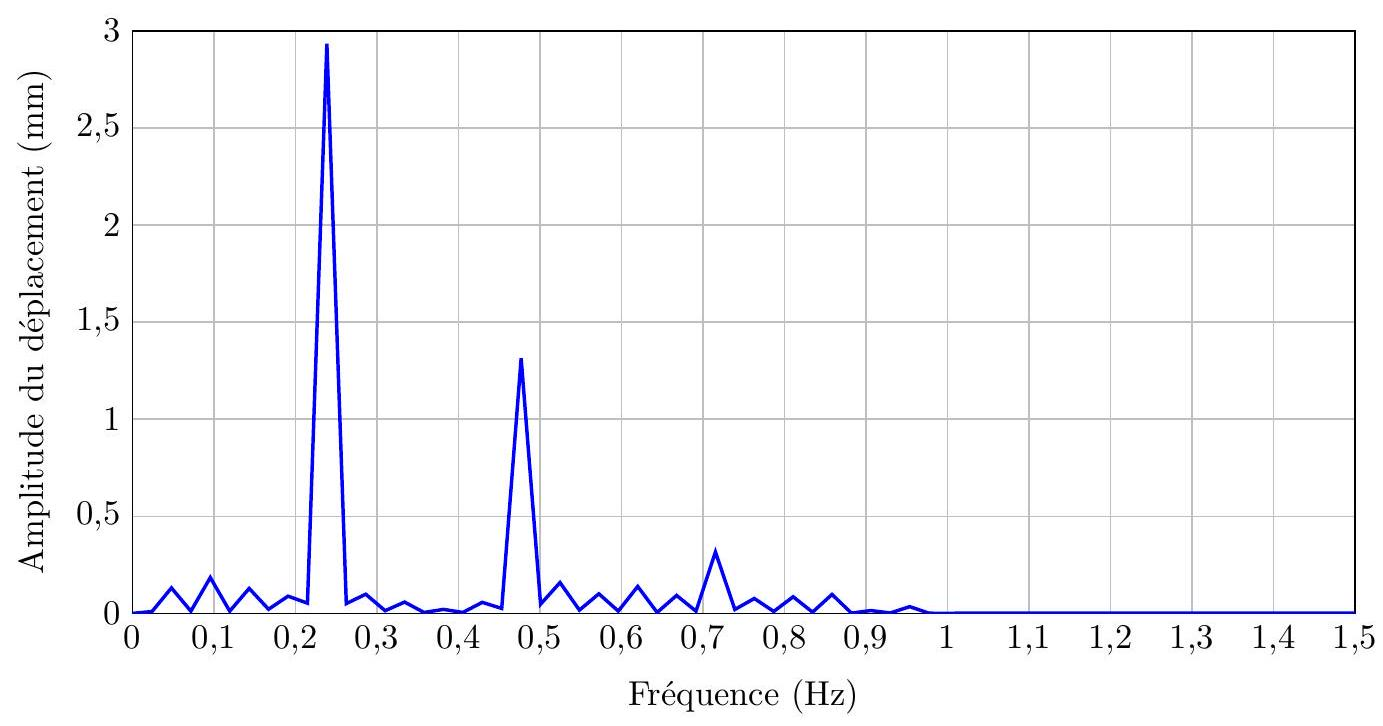
\includegraphics[max width=\textwidth]{2024_08_29_b4f920ed3822451bf72bg-05}
%Figure 5 
\caption{\label{fig_05} Contenu spectral du déplacement dû aux mouvements physiologiques}
\end{figure}


% I.B - 
\section{Cahier des charges partiel de la chaine d'asservissement en position du robot esclave}
%\section{Objectif}
\begin{obj}
Déterminer une valeur numérique pour la bande passante de l'asservissement en position du robot esclave et vérifier le cahier des charges associé.
\end{obj}

Pour cette partie, on retient le modèle de signal de déplacement idéal $z^{*}(t)$ défini précédemment. L'objectif de cette partie est de déterminer la bande passante minimale $\omega_{0 \text { min }}$ en boucle fermée de la chaine d'asservissement permettant d'assurer la précision demandée par le diagramme des exigences.\\
Pour cette pré-détermination, on utilise un modèle simple en raisonnant sur un mouvement selon un seul axe assuré par une chaine d'asservissement (non représentée) dont on note $F(p)$ la fonction de transfert en boucle fermée telle que $F(p)=\frac{Z(p)}{Z^{*}(p)}=\frac{\omega_{0}^{2}}{p^{2}+2 \xi \omega_{0} p+\omega_{0}^{2}}$ où $z^{*}(t)$ est la consigne de déplacement (en mm) et $z(t)$ la sortie de la chaine d'asservissement (en mm). Vis-à-vis de ce signal de consigne, on note l'écart

$$
\varepsilon(t)=z^{*}(t)-z(t)=\varepsilon_{2} \sin \left(2 \pi f_{2} t+\Theta_{2}\right)=\varepsilon_{2} \sin \left(\omega_{2} t+\Theta_{2}\right)
$$

%Q 7. 
\question{On note $H(p)=\frac{\varepsilon(p)}{Z^{*}(p)}$ la fonction de transfert de la consigne $Z^{*}(p)$ vers l'écart $\varepsilon(p)$. Déterminer $H(p)$ en fonction de $\omega_{0}$ et $\xi$. Donner les relations exprimant $\varepsilon_{2}$ et $\Theta_{2}$ en fonction de $\left\|H\left(\mathrm{i} \omega_{2}\right)\right\|$, $\arg \left(H\left(\mathrm{i} \omega_{2}\right)\right), A_{2}$ et $\Phi_{2}$.}
\ifprof
\begin{corrige}

D'une part, $H(p)=\dfrac{\varepsilon (p)}{Z^*(p)}$ et d'autre part, $F(p)=\dfrac{Z (p)}{Z^*(p)}$. Enfin, $\varepsilon(p)=Z^*(p)-Z(p)$. On a donc $\varepsilon(p)=\dfrac{\varepsilon(p)}{H(p)} - F(p)Z^*(p)=\dfrac{\varepsilon(p)}{H(p)} - F(p)\dfrac{\varepsilon(p)}{H(p)}$. On a donc  $\varepsilon(p)=\dfrac{\varepsilon(p)}{H(p)} - F(p)\dfrac{\varepsilon(p)}{H(p)} \Leftrightarrow $ $H(p)=1 - F(p)= p\dfrac{p+2\xi\omega_0  }{p^2+2\xi\omega_0 p + \omega_0^2}$.


En mettant cette fonction de transfert sous forme canonique, on  obtient : 
$
H(p)=\dfrac{2\xi\cdot p}{\omega_0}\dfrac{1+\dfrac{p}{2\xi\omega_0}}{1+\dfrac{2\xi}{\omega_0}p+\dfrac{p^2}{\omega_0^2}}
$.

\begin{itemize}
\item Le module de cette fonction de transfert en remplaçant $p$ par $i\omega$ représente le rapport des amplitudes en régime permanent vis-à-vis d'une entrée $z^*(t)$ sinusoïdale : 
$
\dfrac{\varepsilon_2}{A_2}=\Vert H(i\omega_2)\Vert
$.
\item L'argument de cette fonction de transfert en remplaçant $p$ par $i\omega$ représente le déphasage en régime permanent vis-à-vis d'une entrée $z^*(t)$ sinusoïdale : 
$
\Theta_2-\Phi_2=\arg\left(H(i\omega_2)\right)
$.
\end{itemize}

Ainsi on a : 
$
\left\{
\begin{array}{c}
\varepsilon_2=A_2\cdot \Vert H(i\omega_2)\Vert\\
\\
\Theta_2=\arg\left(H(i\omega_2)\right)+\Phi_2
\end{array}
\right.
$.


%Supposons que  $z_2(t)=A_2\sin \left(\omega_2 t + \Phi_2 \right)$. De plus, $\varepsilon_2(t)=\varepsilon_2 \sin \left( \omega_2 t + \Theta_2 \right)$. On a donc, $\varepsilon_2 = || H\left( i\omega_2\right)|| A_2$, $\Phi_2 - \Theta_2 = \arg \left(H\left(i\omega_2\right)\right)$.



\begin{rem}
Il est peut être souhaitable de préciser avant la question aux candidats qu'on a $z_n(t)=A_n\sin \left(2\pi f_n t + \Phi_n \right)=A_n\sin \left(\omega_n t + \Phi_n \right)$. 
\end{rem}

\end{corrige}
\else
\fi


% Q 8. 
\question{En considérant la bande de pulsations $\omega \ll \omega_{0}$, donner une approximation de $\|H(\mathrm{i} \omega)\|$ sous la forme $\|H(\mathrm{i} \omega)\| \approx K \omega$ où $K$ est un gain à préciser. En considérant cette approximation, donner alors une expression de $\varepsilon_{2}$ en fonction de $A_{2}, \omega_{2}, \omega_{0}$ et $\xi$.}
\ifprof
\begin{corrige}
En considérant de faibles pulsations telles que $\omega\ll \omega_0$, on peut effectuer l'approximation : 
$\Vert H(i\cdot \omega)\Vert\approx\dfrac{2\xi\omega}{\omega_0}$.

On obtient donc bien : $\Vert H(i\omega)\Vert\approx K\cdot \omega $  avec $K=\dfrac{2\xi}{\omega_0}$.

On a alors $\varepsilon_2=A_2\cdot \Vert H(i\omega_2)\Vert $ $\simeq A_2 \dfrac{2\xi}{\omega_0}\omega_2$
\end{corrige}
\else
\fi


%Q 9. 
\question{En considérant $\varepsilon_{2}$, déterminer la valeur minimale de $\omega_{0}$ permettant d'assurer la précision exigée vis-àvis de la consigne sinusoïdale de pulsation $\omega_{2}=2 \pi f_{2}$ (pour l'application numérique, on adoptera un coefficient d'amortissement $\xi=1$ ). Vérifier si l'application numérique est compatible avec celle exprimée par le diagramme des exigences (figure \ref{fig_03} et plus précisément l'exigence 1.2.3).}
\ifprof
\begin{corrige}
D'après l'exigence 1.3.3, $\dfrac{\varepsilon_2}{A_2}<10^{-2}$, on obtient alors la relation suivante : $
\dfrac{\varepsilon_2}{A_2}\approx \dfrac{2\xi\omega_2}{\omega_0}<10^{-2}$.  

Ce qui donne $\omega_0>200\xi\omega_2\approx \SI{603}{rad.s^{-1}}$

L'exigence 1.2 du cahier des charges concernant l'asservissement en position, et donc la fonction de transfert $F(p)$, impose une bande passante (que l'on suppose à $\SI{0}{dB}$), inférieure à $\SI{30}{rad.s^{-1}}$. $F(p)$ est une fonction de transfert du second ordre de gain 1 et la bande passante à $\SI{0}{dB}$ est de l'ordre de $\omega_0\approx \SI{600}{rad.s^{-1}}$. \textbf{Le cahier des charges est donc bien respecté.}
\end{corrige}
\else
\fi


Dans la suite du sujet, il s'agit de déterminer une loi de commande de la chaine d'asservissement permettant d'assurer les exigences du cahier des charges. Cette loi de commande devra résoudre le problème mis en évidence et assurer la compatibilité entre la bande passante minimale et le niveau de précision requis vis-à-vis des consignes sinusoïdales. La conception de cette loi de commande nécessite au préalable de définir et identifier un modèle dynamique du robot esclave, c'est l'objet de la partie suivante.

\section{Analyse géométrique et élaboration du modèle dynamique du robot esclave}
%\section{Objectif}
\begin{obj}
Vérifier la capabilité du robot esclave à respecter le cahier des charges et déterminer le modèle dynamique d'un des axes du robot esclave utilisé pour dimensionner sa commande.
\end{obj}

Ce robot, dont une photo est donnée en figure \ref{fig_06}, est constitué de bras motorisés adaptés à la chirurgie miniinvasive et dispose de quatre mouvements actionnés par des moteurs électriques, dont trois sont visibles sur la figure \ref{fig_06} .

\begin{figure}[!h]
\centering
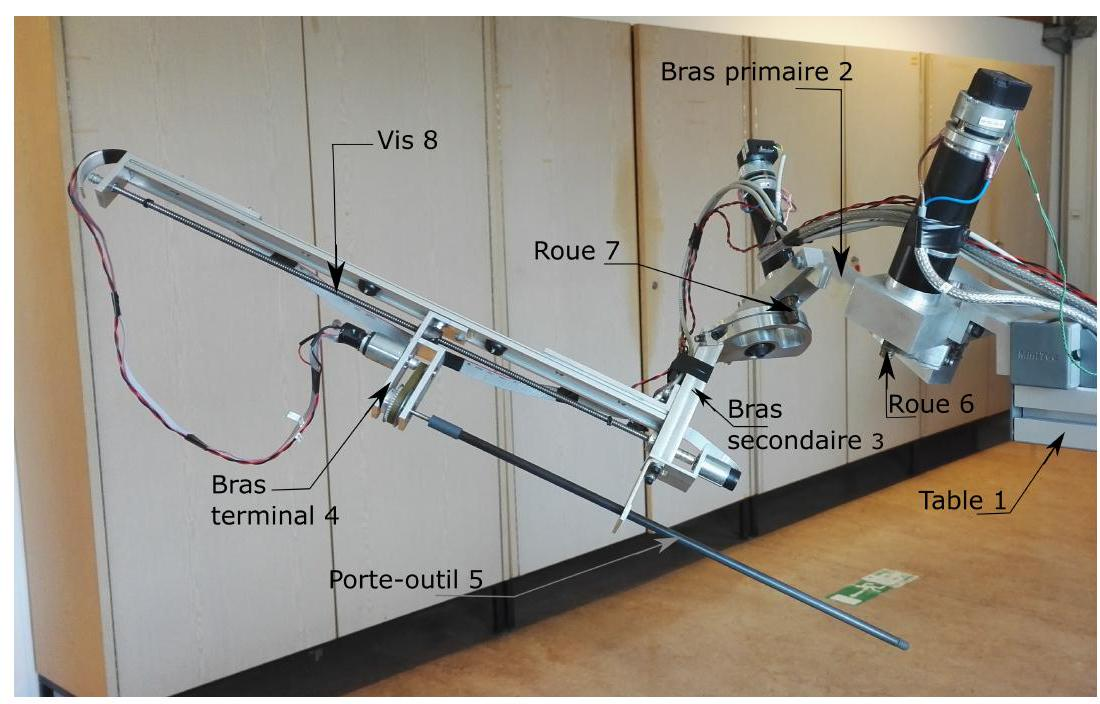
\includegraphics[max width=\textwidth]{2024_08_29_b4f920ed3822451bf72bg-06}
\caption{\label{fig_06}Robot esclave}
\end{figure}

Le schéma cinématique donné en figure \ref{fig_07} est une représentation de la modélisation retenue pour une configuration particulière du robot dans laquelle tous les bras sont coplanaires. Pour ce modèle, le robot est constitué :

\begin{itemize}
  \item d'une table 1 , considérée comme fixe à laquelle on associe un référentiel galiléen $\left(O, \vec{x}_{0}, \vec{y}_{0}, \vec{z}_{0}\right)$, dont $\vec{z}_{0}$ est la verticale ascendante, et un repère $\left(A, \vec{x}_{0}, \vec{y}_{1}, \vec{z}_{1}\right)$, avec $\alpha_{1}=\left(\vec{y}_{0}, \vec{y}_{1}\right)=\left(\vec{z}_{0}, \vec{z}_{1}\right)=\pi / 4 \mathrm{rad}$ et $\overrightarrow{O A}=l_{0} \vec{y}_{0}+l_{1} \vec{y}_{1}$;
  \item d'un bras primaire 2, en liaison pivot d'axe $\left(A, \vec{z}_{1}\right)$ avec la table 1 , auquel on associe un repère $\left(A, \vec{x}_{2}, \vec{y}_{2}, \vec{z}_{1}\right)$, avec $\theta_{21}=\left(\vec{x}_{1}, \vec{x}_{2}\right)=\left(\vec{y}_{1}, \vec{y}_{2}\right)$, et un second repère $\left(B, \vec{x}_{2}{ }^{\prime}, \vec{y}_{2}{ }^{\prime}, \vec{z}_{2}{ }^{\prime}\right)$, avec $\alpha_{2}=\left(\vec{y}_{2}, \vec{y}_{2}{ }^{\prime}\right)=\left(\vec{z}_{1}, \vec{z}_{2}{ }^{\prime}\right)=-\pi / 4 \mathrm{rad}$ et de plus $\overrightarrow{A B}=l_{2} \vec{y}_{2}+l_{2}^{\prime} \vec{y}_{2}{ }^{\prime}$, avec $l_{2}=0,3 \mathrm{~m}$ et $l_{2}^{\prime}=0,44 \mathrm{~m}$;
  \item d'un bras secondaire 3, en liaison pivot d'axe $\left(B, \vec{z}_{2}{ }^{\prime}\right)$ avec le bras primaire 2 , auquel on associe un repère $\left(B, \vec{x}_{3}, \vec{y}_{3}, \vec{z}_{3}\right)$, avec $\theta_{32}=\left(\vec{x}_{2}{ }^{\prime}, \vec{x}_{3}\right)=\left(\vec{y}_{2}{ }^{\prime}, \vec{y}_{3}\right)$
  \item d'un bras terminal 4 , en liaison glissière de direction $\vec{z}_{3}$ avec le bras secondaire 3 . On note $\vec{B} C=l_{3} \vec{y}_{3}+\lambda(t) \vec{z}_{3}$, avec $l_{3}=0,92 \mathrm{~m} ;$
  \item d'un porte-outil 5 , en liaison pivot d'axe $\left(C, \vec{z}_{3}\right)$ avec le bras terminal 4. L'outil lié au porte-outil 5 est caractérisé par le point $D$, désignant le point actif de l'outil (point effectuant l'opération d'incision). On note $\overrightarrow{C D}=l_{4} \vec{z}_{4}$\\
La liaison pivot entre le porte-outil 5 et le bras terminal 4 permet d'obtenir une rotation de l'outil utilisé autour de son axe principal. Elle ne sera pas utilisée dans cette étude, le porte-outil 5 est supposé être immobile par rapport au bras 4 .\\
Les autres mouvements sont générés par des ensembles motoréducteurs:
  \item un premier motoréducteur entraine la roue dentée 6 , qui elle-même entraine une seconde roue dentée liée au bras primaire 2. L'action du motoréducteur sur la roue dentée 6 est modélisée par un couple dont le moment est noté $\vec{C}_{m 1}=C_{m 1} \vec{z}_{1}$
  \item un second motoréducteur entraine l'arbre 7 sur lequel est installé le pignon d'attaque du réducteur 9 . Ce pignon entraine une roue dentée liée au bras secondaire 3 . Le rapport de transmission de ce réducteur 9 est noté $r_{9}$ avec $r_{9}=\frac{\dot{\theta}_{32}}{\dot{\theta}_{72}}=0,25$. Son rendement est noté $\eta_{9}$ avec $\eta_{9}=0,78$. L'action du motoréducteur sur l'arbre 7 est modélisée par un couple dont le moment est noté $\vec{C}_{m 2}=C_{m 2} \vec{z}_{2}{ }^{\prime}$;
  \item enfin, le troisième motoréducteur entraine la vis 8 d'un système vis-écrou dont l'écrou est lié au bras terminal 4. Cette vis est de pas à droite $p=0,63 \mathrm{~mm}$. L'angle de rotation de la vis 8 par rapport au bras secondaire 3 est noté $\theta_{83}$ avec $\theta_{83}=\left(\vec{x}_{3}, \vec{x}_{8}\right)$. L'action du motoréducteur sur la vis 8 est modélisée par un couple dont le moment est noté $\vec{C}_{m 3}=C_{m 3} \vec{z}_{3}$.
\end{itemize}


\begin{figure}[!h]
\centering
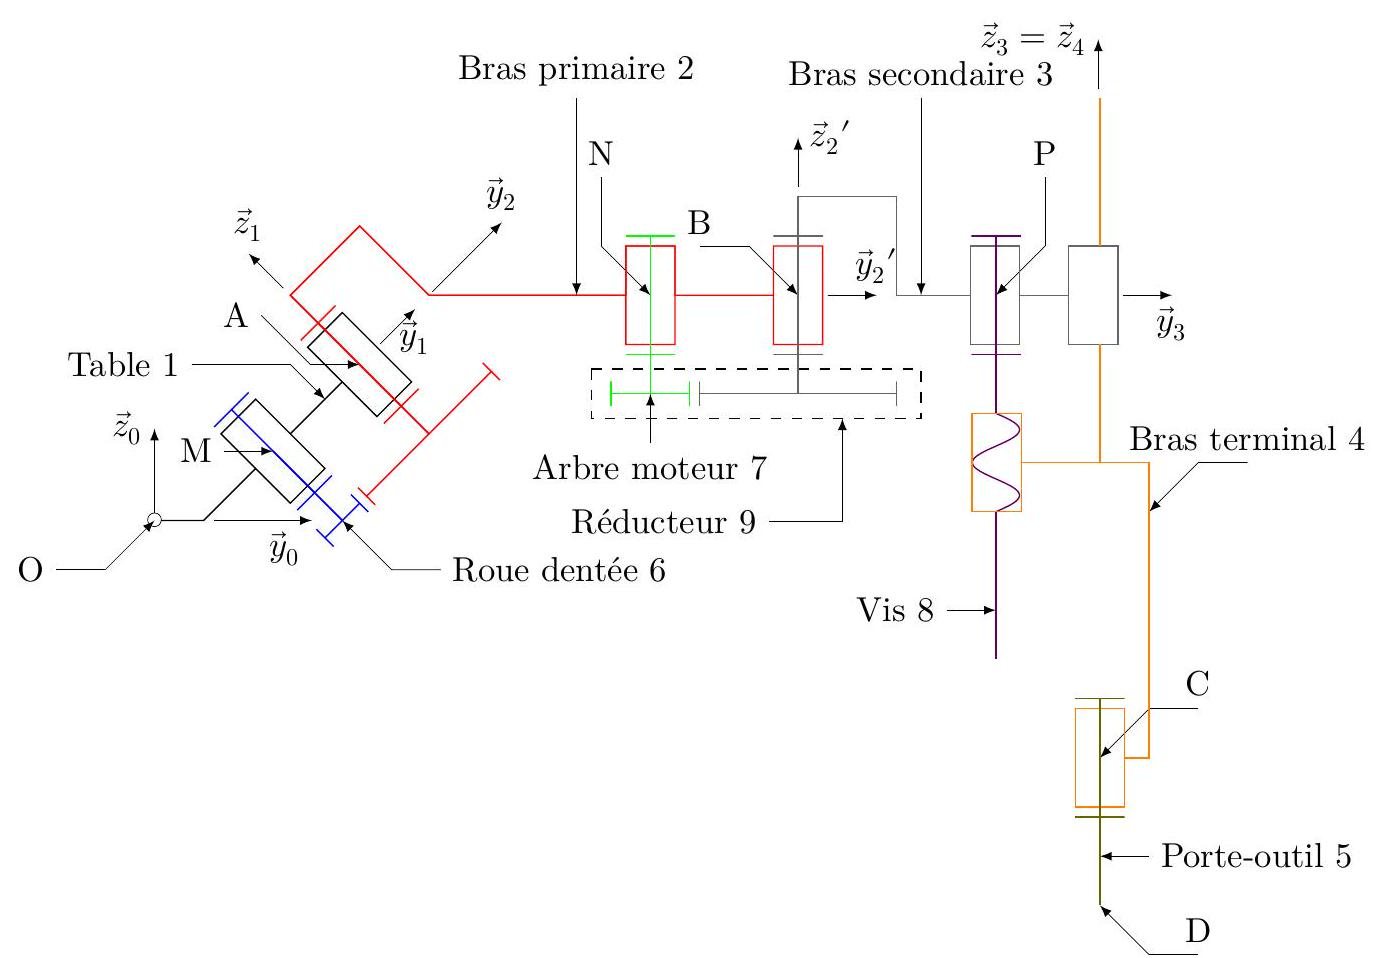
\includegraphics[max width=\textwidth]{2024_08_29_b4f920ed3822451bf72bg-07(1)}
\caption{\label{fig_07} Schéma cinématique 2 D du robot esclave}
\end{figure}

On donne de plus, les caractéristiques suivantes.

\begin{itemize}
  \item Pour le bras secondaire 3
  \item $G_{3}$ son centre de gravité (non représenté sur la figure \ref{fig_07}), défini par $\overrightarrow{B G_{3}}=a_{3} \vec{y}_{3}+b_{3} \vec{z}_{3}$, avec $a_{3}=0,22 \mathrm{~m}$ et $b_{3}=0,15 \mathrm{~m}$;
  \item $J_{3}=6 \times 10^{-1} \mathrm{~kg} \cdot \mathrm{m}^{2}$, son moment d'inertie autour de l'axe $\left(B, \vec{z}_{3}\right)$;
  \item $m_{3}=35,2 \mathrm{~kg}$, sa masse.
  \item Pour le bras terminal 4
  \item $G_{4}$ son centre de gravité (non représenté sur la figure \ref{fig_07}), défini par $\overrightarrow{C G_{4}}=b_{4} \vec{z}_{4}$, avec $b_{4}=0,36 \mathrm{~m}$;
  \item $J_{4}=2,2 \times 10^{-1} \mathrm{~kg} \cdot \mathrm{m}^{2}$, son moment d'inertie autour de l'axe $\left(G_{4}, \vec{z}_{4}\right)$;
  \item $m_{4}=18,4 \mathrm{~kg}$, sa masse.
  \item Les caractéristiques de masse et d'inertie des autres ensembles seront négligées devant celles du bras secondaire 3 et de l'arbre terminal 4 .\\
Le paramétrage angulaire du mécanisme est représenté figure \ref{fig_08}.
\end{itemize}


\begin{figure}[!h]
\centering
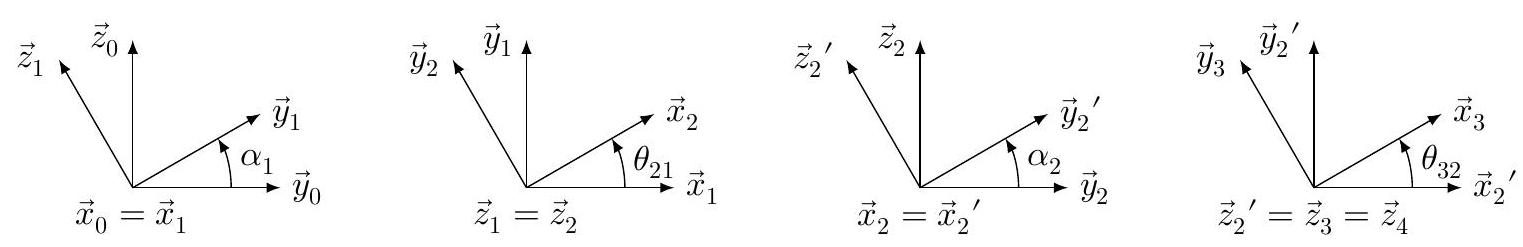
\includegraphics[max width=\textwidth, center]{2024_08_29_b4f920ed3822451bf72bg-07}
\caption{\label{fig_08} Paramétrage angulaire utilisé}
\end{figure}

Afin de déterminer la loi de commande des différents actionneurs, il est nécessaire de connaitre l'influence des différentes actions mécaniques sur le système. On prendra pour la suite de l'étude l'hypothèse que, hormis les liaisons internes au réducteur 9 entre l'arbre moteur 7 et le bras secondaire, les liaisons seront considérées comme parfaites. De plus, on étudiera le robot esclave dans une configuration et pour une commande particulières. En effet, le comportement du système lors de sa phase d'approche de l'organe à opérer est bien moins « sensible » que celui aux alentours de l'organe et lors d'une incision. Ainsi on considérera un mouvement particulier de l'outil chirurgical correspondant à une configuration du robot pré-établie en amont de l'opération. Dans ce cas, on suppose que :

\begin{itemize}
  \item le mouvement relatif entre le bras primaire 2 et la table 1 est nul avec $\dot{\theta}_{21}=0$ et $\theta_{21}=\pi / 3 \mathrm{rad}$. Le point $B$ est alors immobile dans $\left(O, \vec{x}_{0}, \vec{y}_{0}, \vec{z}_{0}\right)$;
  \item à partir d'une position initiale $(t=0)$ de $3 / 2$ telle que $\theta_{32}(t=0)=0$, le mouvement de $3 / 2$ reste de faible amplitude avec $\lambda(t=0)=\lambda_{0}=-0,80 \mathrm{~m}$ et $\theta_{83}(t=0)=0$
  \item le mouvement entre le porte outil 5 et le bras terminal 4 est nul ;
  \item l'action de l'organe opéré sur le porte-outil est négligée devant les autres actions mises en jeu.
\end{itemize}

%II.A - 
\subsection{Vérification de la capabilité du robot esclave}
\begin{obj}
Vérifier la capacité du robot esclave à respecter l'exigence de précision 1.3.3 et dimensionner les capteurs installés sur le robot en conséquence.
\end{obj}

Afin de pouvoir asservir en position le robot esclave, il est nécessaire que la mesure de la position de l'outil soit la plus précise possible. En ce sens, il est nécessaire que la résolution de cette mesure (la plus petite valeur de déplacement mesurable) soit, dans le pire des cas, égale à l'écart maximal autorisé par le cahier des charges.\\
On étudiera uniquement l'influence du robot esclave sur l'écart de position de l'outil. Ainsi, cet écart ne dépend que de la structure cinématique du robot esclave et des capteurs utilisés pour l'asservissement. On considère pour la suite que si le robot esclave est capable de compenser les signaux physiologiques présentés figure \ref{fig_04} en respectant l'exigence 1.3.3 du cahier des charges présenté figure \ref{fig_03}, il sera aussi capable de respecter ce cahier des charges pour la consigne donnée par le chirurgien à l'aide du robot maitre.\\

%Q 10. 
\question{À partir de la figure \ref{fig_04}, déterminer la valeur numérique de $s_{\text {max }}$, la résolution maximale de mesure sur la position de l'outil lors d'une opération pour respecter l'exigence 1.3.3 du cahier des charges présenté figure \ref{fig_03}. La mise en place pré-opératoire définie précédemment permet de considérer que le repère $\left(B, \vec{x}_{2}{ }^{\prime}, \vec{y}_{2}{ }^{\prime}, \vec{z}_{2}{ }^{\prime}\right)$ est un référentiel galiléen. C'est à partir de ce repère que sont définies les trajectoires de l'outil lors de l'opération.}
\ifprof
\begin{corrige}

D'après le cahier des charges $\varepsilon_r<1\%$ (exigence 1.3.3). 
D'après la figure 4, la variation maximale des déplacement est de $\SI{7,5}{mm}$. Il faudrait donc une résolution de $s_{\text{max}}=\SI{75}{\mu m}$.
\end{corrige}
\else
\fi


%Q 11. 
\question{En traduisant la propriété cinématique de la liaison hélicoïdale de pas à droite $p$ et d'axe $\left(P, \vec{z}_{3}\right)$ entre les solides 4 et 8 , donner la relation liant $\lambda(t), \lambda_{0}, p$ et $\theta_{83}$. En déduire l'expression du vecteur position $\overrightarrow{B D}$ caractérisant le point opératoire de l'outil dans la base $\left(\vec{x}_{3}, \vec{y}_{3}, \vec{z}_{3}\right)$ en fonction de $l_{3}, l_{4}, \lambda_{0}, p$ et $\theta_{83}(t)$.}
\ifprof
\begin{corrige}
On a $\lambda(t)=\lambda_0 + \dfrac{p}{2\pi} \theta_{83}(t)$. 
En conséquences, $\vect{BD}=\vect{BC}+\vect{CD}=l_3\vect{y_3}+\lambda(t)\vect{z_3}+l_4\vect{z_4}
=l_3\vect{y_3}+\left( \lambda_0 + \dfrac{p}{2\pi} \theta_{83}(t) \right)\vect{z_3}+l_4\vect{z_3}$.
\end{corrige}
\else
\fi


%Q 12. 
\question{En supposant que $\theta_{32}(t)$ reste de faible amplitude, exprimer les coordonnées $\left(x_{D}, y_{D}, z_{D}\right)$ du vecteur $\overrightarrow{B D}$ dans la base $\left(\vec{x}_{2}{ }^{\prime}, \vec{y}_{2}{ }^{\prime}, \vec{z}_{2}{ }^{\prime}\right)$ en fonction $l_{3}, l_{4}, \lambda_{0}, p, \theta_{32}(t)$ et $\theta_{83}(t)$.}
\ifprof
\begin{corrige}

En projetant $\vect{BD}$ dans la base $\base{x_2'}{y_2'}{z_2'}$, on a 

 $\vect{BD}=l_3\vect{y_3}+\left( \lambda_0 + \dfrac{p}{2\pi} \theta_{83} \right)\vect{z_3}+l_4\vect{z_3}$
 $ =l_3\left( \cos \theta_{32} \vect{y_2'} - \sin\theta_{32} \vect{x_2'}  \right)+\left( \lambda_0 + \dfrac{p}{2\pi} \theta_{83} +l_4\right)\vect{z_2'}$.
 
 Avec l'hypothèse que $\theta_{32}$ reste petit, on a  $\vect{BD}=l_3\left(  \vect{y_2'} - \theta_{32} \vect{x_2'}  \right)+\left( \lambda_0 + \dfrac{p}{2\pi} \theta_{83} +l_4\right)\vect{z_2'}$.
  Ainsi,
  
  $\left(x_D,y_D,z_D\right)=
\left(-l_3 \theta_{32},l_3, \lambda_0 + \dfrac{p}{2\pi} \theta_{83} +l_4\right)$.
\end{corrige}
\else
\fi


Afin de déterminer la résolution de mesure $s_{D}$ sur le déplacement du point $D$, il est choisi d'utiliser une hypothèse de propagation quadratique des incertitudes avec un coefficient de sécurité de 3 . Ainsi, on peut écrire

$$
s_{D}=3 \sqrt{s_{X}^{2}+s_{Y}^{2}+s_{Z}^{2}}
$$

où $s_{X}, s_{Y}$ et $s_{Z}$ sont les résolutions de mesure respectivement suivant les directions $\vec{x}_{2}{ }^{\prime}, \vec{y}_{2}{ }^{\prime}$ et $\vec{z}_{2}{ }^{\prime}$.\\
Afin de réaliser l'asservissement du robot esclave, deux capteurs identiques permettant la mesure des angles $\theta_{32}$ et $\theta_{83}$ ont été mis en œuvre. On note la résolution de ces capteurs $s_{\text {capteur }}$.\\

%Q 13. 
\question{Exprimer $s_{D}$ en fonction de $l_{3}$, $p$, et la résolution de mesure sur les angles $s_{\text {capteur }}$. En déduire la valeur maximale de $s_{\text {capteur }}$ pour pouvoir respecter l'exigence 1.3.3 du cahier des charges.}
\ifprof
\begin{corrige}
Soit, $s_D=3\sqrt{s_X^2+s_Y^2+s_Z^2}$. Par calcul différentiel :  \textcolor{red}{XP?}

\begin{minipage}{0.5\textwidth}
\begin{align*}
\left\{
\begin{array}{c}
dx_D=-l_3d\theta_{32}\\
dy_D=0\\
dz_D=\dfrac{p}{2\pi}d\theta_{83}
\end{array}
\right.
\end{align*}
\end{minipage}
\begin{minipage}{0.5\textwidth}

\begin{align*}
\left\{
\begin{array}{c}
s_X=\Delta x_D=l_3\Delta \theta_{32}=l_3 s_{\text{capteur}}\\
s_Y=\Delta y_D=0\\
s_Z=\Delta z_D=\dfrac{p}{2\pi}\Delta \theta_{83}=\dfrac{p}{2\pi}s_{\text{capteur}}
\end{array}
\right.
\end{align*}
\end{minipage}

Ainsi,$
s_D=3\cdot s_{\text{capteur}}\sqrt{l_3^2+\dfrac{p^2}{4\pi^2}}
$.
Le cahier des charges impose la relation suivante,

$
s_{\text{capteur}}<\dfrac{75\mu m}{3\sqrt{l_3^2+\dfrac{p^2}{4\pi^2}}}
$.

L'application numérique donne pour résolution maximale afin de respecter le cahier des charge :  $s_{\text{capteur}}=2,72\times \SI{e-5}{}$.
\end{corrige}
\else
\fi


%II.B - 
\subsection{Détermination et vérification du modèle dynamique du robot esclave}
\begin{obj}
Déterminer le modèle dynamique du robot esclave en vue de l'élaboration de sa commande.
\end{obj}
%II.B.1)
\subsubsection{Vérification du fonctionnement du réducteur 9}
Le réducteur 9 , monté entre l'arbre moteur 7 et le bras secondaire 3 , représenté sur la figure \ref{fig_07} par un ensemble de deux roues dentées est en fait un train épicycloïdal. L'action de l'arbre de sortie de ce réducteur sur le bras secondaire est modélisée par un couple dont le moment est noté $\vec{C}_{73}=C_{73} \vec{z}_{2}{ }^{\prime}$.

On se propose de vérifier les caractéristiques du réducteur fournies par le constructeur (rendement et rapport de transmission) dans l'optique de l'élaboration du modèle dynamique du robot.

%Q 14. 
\question{Exprimer $\vec{C}_{73}$, le moment de l'action mécanique exercée par l'arbre moteur 7 sur le bras secondaire 3 en B, en fonction de $C_{m 2}, r_{9}$ et $\eta_{9}$.}
\ifprof
\begin{corrige}
On se place en régime permanent. Le rendement peut s'exprimer par 
$\eta_9 =\dfrac{C_{73}\dot{\theta}_{32}}{C_{m2}\dot{\theta}_{72}}=\dfrac{C_{73}}{C_{m2}}r_9$. 
On a donc, en régime permanent, $\vect{C_{73}}=C_{73}\vect{z'_2}=C_{m2}\dfrac{\eta_9}{r_9}\vect{z'_2}$.


\textbf{Remarque :} peut-être aurait-il été souhaitable de préciser que l'on souhaite cette relation en régime permanent ?
\end{corrige}
\else
\fi


Un essai sur le réducteur 9 a permis d'obtenir la courbe figure \ref{fig_09} représentant l'évolution du couple en sortie du réducteur $C_{73}$ en fonction du couple en entrée $C_{m 2}$.\\
%Q 15. 
\question{Conclure sur la validité des valeurs de $r_{9}$ et $\eta_{9}$ fournies par le constructeur.}
\ifprof
\begin{corrige}
Au vu du tracé expérimental de $C_{73}$ en fonction de $C_{m2}$, on peut réaliser une linéarisation sur l'intervalle $[0,10]$ et $C_{73}\simeq 3 C_{m2}$. 
D'après les données constructeur, on a $C_{73}=C_{m2}\dfrac{\eta_9}{r_9}=C_{m2}\dfrac{0,78}{0,25}=\SI{3,12}{Nm}$.

On peut donc valider les valeurs données par le constructeur.
\end{corrige}
\else
\fi


% II.B.2) 
\subsubsection{Élaboration du modèle dynamique d'un axe du robot esclave}
Le graphe de structure de la modélisation retenue pour le système est donné sur la figure \ref{fig_A} du document réponse.\\
%Q 16. 
\question{Sur la figure \ref{fig_A}, donner le nombre d'inconnues d'actions mécaniques (noté NI-AM) pour chacune des liaisons représentées sur le graphe de structure et indiquer les actions extérieures auxquelles sont soumises les différentes classes d'équivalence cinématiques.}
\ifprof
\begin{corrige}
\begin{center}
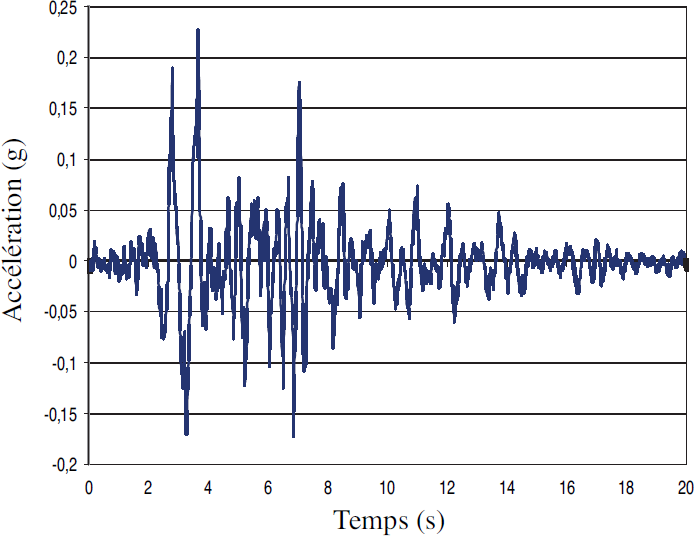
\includegraphics[width=\textwidth]{fig_02}
\end{center}

\textbf{Remarque :} en ajoutant l'hypothèse en début de partie II.B.1, l'action de 7 sur 3 est modélisée par un couple. Dans ce cas, le résultat attendu est peut-être 1 inconnue entre 7 et 3.
\end{corrige}
\else
\fi


%Q 17. 
\question{Proposer, le plus clairement et synthétiquement possible, sans calcul, une démarche qui permette d'exprimer le couple nécessaire $C_{m 2}$ à fournir sur l'arbre 7 du motoréducteur afin de réaliser le mouvement décrit précédemment.}
\ifprof
\begin{corrige}
On cherche à déterminer le couple $C_{m2}$ à fournir sur l'arbre 7. L'arbre 7 est en rotation autour de l'axe $\axe{N}{z_2'}$. Il entraîne l'ensemble $\left\{3+8+4+5\right\}$ en rotation autour de l'axe $\axe{B}{z_2'}$.

\begin{center}
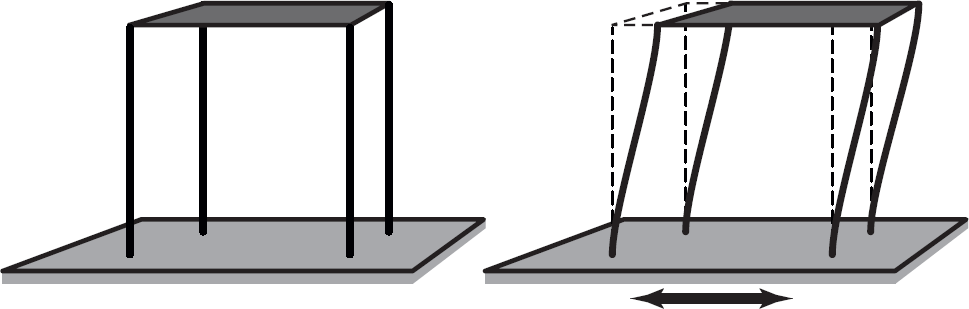
\includegraphics[width=\textwidth]{fig_05}
\end{center}

On propose donc les isolements et des théorèmes associés suivants : 
\begin{itemize}
\item isolement de $\left\{3+8+4+5\right\}$ : théorème du moment dynamique en projection sur $\left(B,\overrightarrow{z}_2'\right)$ qui permet de relier l'action de 7 sur 3 aux paramètres de mouvement de l'ensemble $\left\{3+8+4+5\right\}$ qui représente dans le cas particulier du mouvement souhaité la même classe d'équivalence;
\item isolement de $7$ : théorème du moment dynamique selon $\left(N,\overrightarrow{z}_2'\right)$ qui revient à un théorème du moment statique car l'inertie de 7 est négligeable. Cela permet de relier $C_{m2}$ à l'action de 3 sur 7.
\end{itemize}
Cet ordonnancement des isolements permet de ne pas faire apparaître les inconnues dans les liaisons pivot entre 2 et 7 ainsi qu'entre 7 et 3. 
\end{corrige}
\else
\fi



\begin{figure}[!h]
\centering
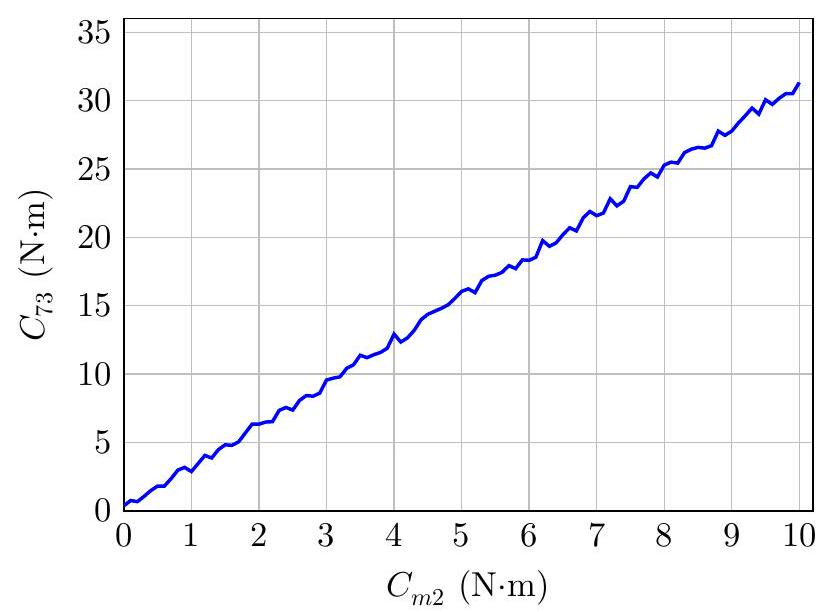
\includegraphics[max width=.7\textwidth]{2024_08_29_b4f920ed3822451bf72bg-09(1)}
\caption{\label{fig_09} Évolution de $C_{73}$ en fonction de $C_{m 2}$}
\end{figure}

%Q 18. 
\question{Exprimer $\vec{V}_{G_{4}, 4 / 1}$ la vitesse du point $G_{4}$ centre de gravité du bras terminal 4 dans son mouvement par rapport à la table 1 , en fonction de $l_{3}, \dot{\lambda}$ et $\dot{\theta}_{32}$.\\
Un essai a permis d'obtenir le relevé de mesure présenté figure \ref{fig_10} pour une loi de commande de $\theta_{32}(t)$ en trapèze de vitesse. On supposera que le temps de réponse du moteur est tel que l'évolution de la vitesse suit parfaitement son profil de commande.}
\ifprof
\begin{corrige}
On cherche $\vectv{G_4}{4}{1}$. On a $\vect{OG_4}=\vect{OA}+\vect{AB}+\vect{BC}+\vect{CG_4}$ $=l_0\vect{y_0}+l_1\vect{y_1}+l_2\vect{y_2}+l_2'\vect{y_2'}+l_3\vect{y_3}+\lambda(t)\vect{z_3}+b_4\vect{z_4}$.
On a $\alpha_1=\dfrac{\pi}{4}$ et $\alpha_2=-\dfrac{\pi}{4}$.

On a donc $\vectv{G_4}{4}{1}= \left[\dfrac{\dd \vect{OG_4}}{\dd t}\right]_{\rep{0}} $ 

$= 
\left[\dfrac{\dd l_0\vect{y_0}}{\dd t}\right]_{\rep{0}}+
\left[\dfrac{\dd l_1\vect{y_1}}{\dd t}\right]_{\rep{0}}+
\left[\dfrac{\dd l_2\vect{y_2}}{\dd t}\right]_{\rep{0}}+
\left[\dfrac{\dd l_2'\vect{y_2'}}{\dd t}\right]_{\rep{0}}+
\left[\dfrac{\dd l_3\vect{y_3}}{\dd t}\right]_{\rep{0}}+
\left[\dfrac{\dd \lambda(t)\vect{z_3}}{\dd t}\right]_{\rep{0}}+
\left[\dfrac{\dd b_4\vect{z_4}}{\dd t}\right]_{\rep{0}}$

$= 
\vect{0}+
\vect{0}+
l_2\left[\dfrac{\dd \vect{y_2}}{\dd t}\right]_{\rep{0}}+
l_2'\left[\dfrac{\dd \vect{y_2'}}{\dd t}\right]_{\rep{0}}+
l_3\left[\dfrac{\dd \vect{y_3}}{\dd t}\right]_{\rep{0}}+
\lambda(t)\left[\dfrac{\dd \vect{z_3}}{\dd t}\right]_{\rep{0}}+
\dot{\lambda}(t)\left[\dfrac{\dd \vect{z_3}}{\dd t}\right]_{\rep{0}}+
b_4\left[\dfrac{\dd \vect{z_4}}{\dd t}\right]_{\rep{0}}$

$= 
l_2\left[ \vecto{2}{0} \wedge \vect{y_2} \right]+
l_2'\left[ \vecto{2'}{0} \wedge \vect{y_2'} \right]+
l_3\left[ \vecto{3}{0} \wedge \vect{y_3} \right]+
\lambda(t)\left[ \vecto{3}{0} \wedge \vect{z_3} \right]+
\dot{\lambda}(t)\vect{z_3}+
b_4\left[ \vecto{4}{0} \wedge \vect{z_4} \right]$. 

$= 
l_2\left[ \dot{\theta}_{21}\vect{z_2} \wedge \vect{y_2} \right]+
l_2'\left[ \dot{\theta}_{21}\vect{z_2} \wedge \vect{y_2'} \right]+
l_3\left[ \left(\dot{\theta}_{21}\vect{z_2}+\dot{\theta}_{32}\vect{z_3} \right) \wedge \vect{y_3} \right]+
\lambda(t)\left[ \left(\dot{\theta}_{21}\vect{z_2}+\dot{\theta}_{32}\vect{z_3} \right) \wedge \vect{z_3} \right]+
\dot{\lambda}(t)\vect{z_3}+
b_4\left[ \left(\dot{\theta}_{21}\vect{z_2}+\dot{\theta}_{32}\vect{z_3} \right) \wedge \vect{z_3} \right]$. 

Or $\dot{\theta}_{21}=0$. On a donc :
$\vectv{G_4}{4}{1}= 
l_3\left(\dot{\theta}_{32}\vect{z_3} \wedge \vect{y_3} \right)+
\dot{\lambda}(t)\vect{z_3} =
-\dot{\theta}_{32}l_3\vect{x_3}  + \dot{\lambda}(t)\vect{z_3}$.
\end{corrige}
\else
\fi



\begin{figure}[!h]
\centering
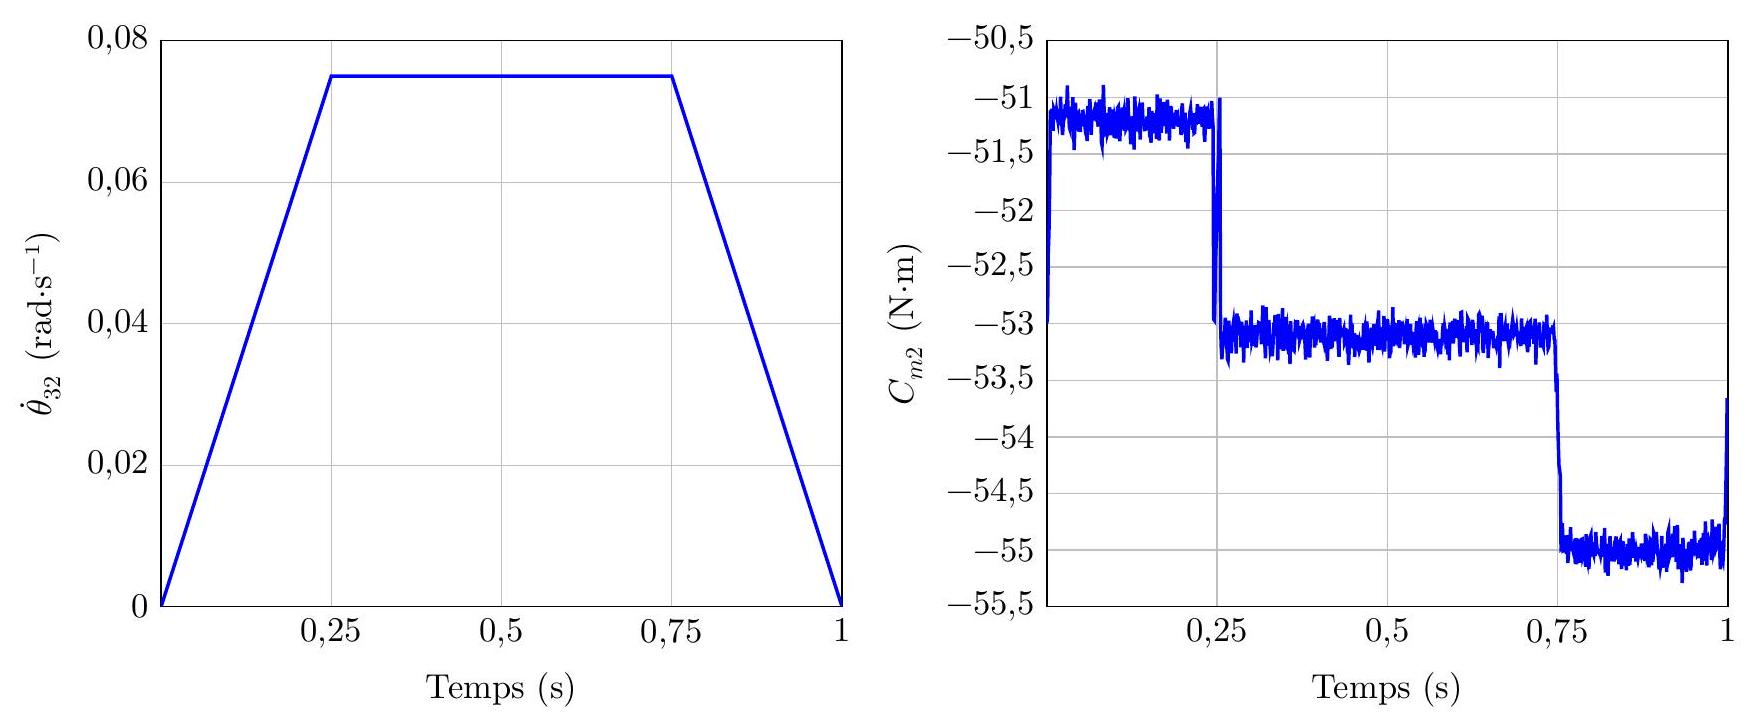
\includegraphics[max width=\textwidth]{2024_08_29_b4f920ed3822451bf72bg-09}
\caption{\label{fig_10} Évolution de $\dot{\theta}_{32}$ et de $C_{m 2}$}
\end{figure}

%Q 19. 
\question{Justifier l'hypothèse que la valeur de $\theta_{32}(t)$ reste faible. En déduire que l'on pourra considérer pour la suite que}
$$
\forall t, \quad \cos \left(\theta_{32}(t)\right) \approx 1 \quad \text { et } \quad \sin \left(\theta_{32}(t)\right) \approx 0
$$
\ifprof
\begin{corrige}
En utilisant l'évolution de $\dot{\theta}_{32}$, on peut déterminer le déplacement angulaire effectué en traçant l'aire sous la courbe :
$\theta_{32}=\dfrac{1}{2}\left( 1+0,5\right)\times 0,075 =\SI{0,056}{rad}\simeq 3^{\text{o}}$.

Cet angle étant faible, on peut donc considérer que $\forall t \cos \left(\theta_{32}(t)\right)\simeq 1$ et $\sin\left(\theta_{32}(t)\right)\simeq 0$.
\end{corrige}
\else
\fi


%Q 20. 
\question{Exprimer $\vec{\delta}_{B, 4 / 1} \cdot \vec{z}_{4}$, la projection du moment dynamique au point $B$ appartenant au bras terminal 4 dans son mouvement par rapport à la table 1 sur la direction $\vec{z}_{4}$, en fonction de $J_{4}, m_{4}, l_{3}$ et $\ddot{\theta}_{32}$.}
\ifprof
\begin{corrige}
On donne $J_4$ le moment d'inertie du bras 4 autour de l'axe $\axe{G_4}{z_4}$.

\textbf{Méthode}
\begin{enumerate}
\item Expression de $\vectmd{B}{4}{1}\cdot\vect{z_4} = \left( \vectmd{G_4}{4}{1} + \vect{BG_4}\wedge m_4 \vectg{G_4}{4}{1}\right)\cdot\vect{z_4}$.
\item Calcul de $\vectmd{G_4}{4}{1}$.
\end{enumerate}

$\vectmd{G_4}{4}{1} \cdot\vect{z_4} = \left[ \dfrac{\dd \vectmc{G_4}{4}{1}}{\dd t} \right]_{\rep{0}}\cdot\vect{z_4}
=\left[ \dfrac{\dd \vectmc{G_4}{4}{1}\cdot \vect{z_4}}{\dd t} \right]-\vectmc{G_4}{4}{1}\cdot\left[ \dfrac{\dd \vect{z_4}}{\dd t} \right]_{\rep{0}}$



On a $\vectmc{G_4}{4}{1} =\inertie{G_4}{4} \vecto{4}{1}$ avec $\vecto{4}{1}=\underbrace{\vecto{4}{3}}_{\vect{0}}+\vecto{3}{2}+\vecto{2}{1} =\dot{\theta}_{32} \vect{z_3}+\underbrace{\dot{\theta}_{21}}_{0} \vect{z_2}=\dot{\theta}_{32} \vect{z_4}$.

Donc,
$\vectmc{G_4}{4}{1}\cdot\vect{z_4}=J_4\dot{\theta}_{32} $.

De plus, $ \left[ \dfrac{ \dd \vect{z_4}}{\dd t} \right]_{\rep{0}} = \vect{0} $. 
En conséquences, $\vectmd{G_4}{4}{1} \cdot\vect{z_4}  = J_4\ddot{\theta}_{32}$.

Par ailleurs, $\vectg{G_4}{4}{1}= \left[\dfrac{\dd \vectv{G_4}{4}{1}}{\dd t} \right]_{\rep{0}}=\left[\dfrac{\dd \left( -\dot{\theta}_{32}l_3\vect{x_3}  + \dot{\lambda}(t)\vect{z_3} \right)}{\dd t} \right]_{\rep{0}}$
$= -\ddot{\theta}_{32}l_3\vect{x_3} -\dot{\theta}_{32}l_3    \left(\dot{\theta}_{32} \vect{z_3}\wedge \vect{x_3} \right)  + \ddot{\lambda}(t)\vect{z_3}  $

$= -\ddot{\theta}_{32}l_3\vect{x_3} -l_3   \dot{\theta}_{32}^2  \vect{y_3} + \ddot{\lambda}(t)\vect{z_3}  $.

$\left(\vect{BG_4}\wedge m_4 \vectg{G_4}{4}{1}\right)\cdot\vect{z_4} = 
m_4\left( \left(l_3 \vect{y_3} + \lambda(t) \vect{z_3}+ b_4 \vect{z_4}\right) \wedge  \left(-\ddot{\theta}_{32}l_3\vect{x_3} -l_3   \dot{\theta}_{32}^2  \vect{y_3} + \ddot{\lambda}(t)\vect{z_3} \right) \right)\cdot \vect{z_{4,3}}$

Par simplification avec les propriétés du produit mixte et du produit vectoriel,

$
\left(\vect{BG_4}\wedge m_4 \vectg{G_4}{4}{1}\right)\cdot\vect{z_4} =
m_4\left( \left(l_3 \vect{y_3} \right) \wedge  \left(-\ddot{\theta}_{32}l_3\vect{x_3} \right) \right)\cdot \vect{z_{4,3}}
=m_4\cdot l_3^2\ddot{\theta}_{32}
$


  Au final,  $\vectmd{B}{4}{1}\cdot\vect{z_4} = J_4 \ddot{\theta}_{32}+\ddot{\theta}_{32}l_3^2 m_4 $.

\end{corrige}
\else
\fi


%Q 21. 
\question{En appliquant le principe fondamental de la dynamique, exprimer le couple $C_{m 2}$ sous la forme}
$$
\indice{J}{eq} \ddot{\theta}_{32}(t)=A C_{m 2}(t)+C_{r}(t)
$$

Donner alors l'expression littérale, puis la valeur numérique de

\begin{itemize}
  \item $\indice{J}{eq}$ en fonction de $J_{3}, J_{4}, m_{4}$ et $l_{3}$;
  \item $A$ en fonction de $r_{9}$ et $\eta_{9}$
  \item $C_{r}(t)$ en fonction de $g$ (accélération de la pesanteur), $m_{3}, m_{4}, a_{3}, l_{3}, \alpha_{1}$ et $\theta_{21}$.
\end{itemize}

\ifprof
\begin{corrige}
Par analogie avec la question précédente, on a $\vectmd{B}{3}{1}\cdot\vect{z_4}= J_3\ddot{\theta}_{32}+\ddot{\theta}_{32}a_3^2 m_3$.

En conséquence,  $\vectmd{B}{3+4+5+8}{1}\cdot\vect{z_4} = \left(J_3+J_4+a_3^2 m_3  +l_3^2 m_4\right) \ddot{\theta}_{32}$.

\begin{rem}
On fait l'hypothèse ici que l'action de 3 sur 7 ou du réducteur sur 7 est bien modélisée par une action mécanique de type couple comme le suggère l'énoncé.
\end{rem}



\textbf{On isole l'ensemble $\{3,4,5,8\}$.}

\begin{rem}
Le schéma peut être trompeur car représenté dans une configuration particulière mais la pesanteur crée un moment en $B$ suivant $\vect{z_0}$.
\end{rem}

\begin{itemize}
\item On réalise le bilan des actions mécaniques extérieures. 
\begin{itemize}
\item Action de la pesanteur sur 3 : 
$\vectm{B}{\text{pes}}{3}\cdot \vect{z_4} $ $ =\left(\vect{BG_3}\wedge \left(-m_3g \vect{z_0}\right) \right)\vect{z_4}$ 
$ =\left(\left( a_3\vect{y_3} + b_3\vect{z_3}  \right)\wedge \left(-m_3g \vect{z_0}\right)\right)\vect{z_4}$
$ =\left( a_3\vect{y_4} \wedge \left(-m_3g \vect{z_0}\right)\right)\vect{z_4}$
$ =\left( \vect{z_4} \wedge a_3\vect{y_4}\right)\cdot  \left(-m_3g \vect{z_0}\right)$
$ = a_3 m_3g \left( \vect{x_3}\cdot \vect{z_0} \right)$
$ = a_3 m_3g \left(  \cos\theta_{32} \vect{x_2'} +\sin\theta_{32} \vect{y_2'} \right)\cdot \vect{z_0} $

On utilise les hypothèses de linéarisation vues précédemment et on a 
$\vectm{B}{\text{pes}}{3}\cdot \vect{z_4}= a_3 m_3g \vect{x_2'} \cdot \vect{z_0} $ 
$= a_3 m_3g \vect{x_2} \cdot \vect{z_0} $
$= a_3 m_3g \left( \cos \theta_{21} \vect{x_1} +\sin \theta_{21} \vect{y_1} \right)\cdot \vect{z_0} $
$= a_3 m_3g \left( \cos \theta_{21} \vect{x_0} +\sin \theta_{21}  \left( \cos \alpha_1 \vect{y_0} + \sin \alpha_1 \vect{z_0} \right) \right)\cdot \vect{z_0} $
$= a_3 m_3g \sin \theta_{21}   \sin \alpha_1    $. En faisant l'application numérique, on a donc 
$\vectm{B}{\text{pes}}{3}\cdot \vect{z_4}= a_3 m_3g  \dfrac{\sqrt{2}}{2} \dfrac{\sqrt{3}}{2}$

\item Action de la pesanteur sur 4 : 
$\vectm{B}{\text{pes}}{4}\cdot \vect{z_4} $ $ =\left(\vect{BG_4}\wedge \left(-m_4g \vect{z_0}\right) \right)\vect{z_4}$ 

$ =\left(\left(l_3\vect{y_3} + \lambda(t) \vect{z_{3,4}} + b_4\vect{z_{3,4}} \right)\wedge \left(-m_4g \vect{z_0}\right) \right)\vect{z_{3,4}}
=\overrightarrow{z}_{3,4}\wedge l_3\overrightarrow{y}_3\cdot \left(-m_4\cdot g\cdot \overrightarrow{z}_0\right)=m_4l_3g\overrightarrow{x}_3\cdot \overrightarrow{z}_0
$

Or,

$\overrightarrow{x}_3=\cos\theta_{32}\overrightarrow{x}_{2,2'}+\sin\theta_{32}\overrightarrow{y}_{2'}$

avec $\cos\theta_{32}\approx 1$ et $\sin\theta_{32}\approx 0$

 Donc, 
 
 $\overrightarrow{x}_3\cdot \overrightarrow{z}_0=\left(\cos\theta_{21}\overrightarrow{x}_{1,0}+\sin\theta_{21}\overrightarrow{y}_1\right)\cdot \overrightarrow{z}_0=\sin\theta_{21}\sin\alpha_1=\dfrac{\sqrt{6}}{4}$
 On obtient alors,
 
 $\vectm{B}{\text{pes}}{4}\cdot \vect{z_4} = =l_3 m_4g\sin\theta_{21}\sin\alpha_1 =l_3 m_4g  \dfrac{\sqrt{6}}{4}$.

\item $\vectm{B}{2}{3}\cdot \vect{z_0}=0$.
\item $\vectm{B}{7}{3}\cdot \vect{z_4}=C_{73}$ (Indication du sujet).
\end{itemize}
\item En appliquant le théorème du moment dynamique en $B$ en projection sur $\vect{z}$ on a donc 
$  \left( a_3^2 m_3  +l_3^2 m_4+J_3+J_4\right) \ddot{\theta}_{32}=C_{73} + g  \sin \theta_{21}   \sin \alpha_1 \left( a_3 m_3 + l_3 m_4\right) $.
\end{itemize}

\textbf{Il semblerait que ce qui est attendu soit d'utiliser ${C_{73}}=C_{m2}\dfrac{\eta_9}{r_9}$, mais cette relation avait été établie en régime permanent ce qui n'est plus le cas. } 


$\left(J_3+J_4  + a_3^2 m_3  +l_3^2 m_4 \right) \ddot{\theta}_{32} =C_{m2}\dfrac{\eta_9}{r_9}+ g  \sin \theta_{21}   \sin \alpha_1 \left( a_3 m_3 + l_3 m_4\right) $.

Par identification, on a donc :
\begin{itemize}
\item $\indice{J}{eq} = J_3+J_4  + a_3^2 m_3  +l_3^2 m_4$;
\item $A  =\dfrac{\eta_9}{r_9}$;
\item $C_r(t)=g  \sin \theta_{21}   \sin \alpha_1 \left( a_3 m_3 + l_3 m_4\right) $.
\end{itemize}

\begin{rem} 
$\indice{J}{eq}$ dépendrait aussi de $a_3$ et $m_3$.
\end{rem}
\end{corrige}
\else
\fi


%Q 22.
\question{À partir de la figure \ref{fig_10}, déterminer les valeurs expérimentales du couple résistant $C_{r}(t)$ et de l'inertie équivalente $J_{\text {eq }}$ ramenée sur l'axe $\left(B, \vec{z}_{3}\right)$.}
\ifprof
\begin{corrige}
\begin{itemize}
\item \textbf{Méthode 1 : }
D'après l'expression donnée, on a $C_r(t)=\indice{J}{eq}\ddot{\theta}_{32}(t)-A C_{m2}(t)$.
Lorsque la vitesse est constante, on a donc $C_r(t)=-A C_{m2}(t)$ avec $C_{m2}(t)=-\SI{53,25}{Nm}$ et 
$C_r(t)= \dfrac{0,78}{0,25} \cdot  53,25  = \SI{166,14}{Nm}$.   \textbf{Trop grand.}


À accélération constante, $\ddot{\theta}_{32} = \dfrac{0,075}{0,25}=\SI{0,3}{rad.s^{-2}}$. 

On a donc 
$\indice{J}{eq}=\dfrac{C_r(t)+A C_{m2}(t)}{\ddot{\theta}_{32}(t)}=\dfrac{C_r(t)-A 51,25}{0,3}$ 
$\dfrac{166,14  -51,25\dfrac{0,78}{0,25}}{0,3}=\SI{20,8}{kg.m^2}$. 

\item \textbf{Méthode 2 : }
Soit,
\begin{itemize}
\item $C^{a}_{m2}=C_{m2}(t)\approx-\SI{51,2}{Nm}$ pour $t\in\left[0;0,25\right]$ ;
\item $C^{b}_{m2}=C_{m2}(t)\approx-\SI{53}{Nm}$ pour $t\in\left[0,25;0,75\right]$ ;
\item $C^{b}_{m2}=C_{m2}(t)\approx-\SI{55}{Nm}$ pour $t\in\left[0,75;1\right]$ ;
\item $\ddot{\theta}_{32}(t)=\ddot{\theta}_{32a}=\dfrac{0,075}{0,25}=\SI{0,3}{rad. s^{-2}}$ pour $t\in \left[0;0,25\right]$
\end{itemize}

On obtient alors 3 équations : 
$
\left\{
\begin{array}{l}
\indice{J}{eq}\ddot{\theta}_{32a}=A\cdot C^{a}_{m2}+C_r(t) \quad (a)\\
0=A\cdot C^{b}_{m2}+C_r(t)  \quad (b)\\
-\indice{J}{eq}\ddot{\theta}_{32a}=A\cdot C^{c}_{m2}+C_r(t)  \quad (c)\\
\end{array}
\right.
$

En combinant les équations : 
\begin{itemize}
\item $(b) \rightarrow C_r(t)=-A\cdot  C^{b}_{m2}=-\dfrac{\eta_9}{r_9}C^{b}_{m2}\approx \SI{165,67}{Nm}$
\item $(a)-(c)\rightarrow 2 \indice{J}{eq} \ddot{\theta}_{32a}=A\cdot \left(C^{a}_{m2}-C^{c}_{m2}\right)$
\end{itemize}

On obtient alors,

\begin{align*}
\indice{J}{eq}=\dfrac{A\cdot \left(C^{a}_{m2}-C^{c}_{m2}\right)}{2\ddot{\theta}_{32a}} \approx \SI{19,76}{kg}\cdot m^2
\end{align*}
\end{itemize}
\end{corrige}
\else
\fi


%Q 23. 
\question{À partir de la figure \ref{fig_10}, en comparant les valeurs théoriques et expérimentales de l'inertie équivalente et du couple résistant ramenés sur l'arbre 7 du motoréducteur, expliquer les écarts éventuels et conclure sur la validité du modèle utilisé.}
\ifprof
\begin{corrige}
En faisant l'application numérique à partir des données de l'énoncé, on trouve : 

$
\left\{
\begin{array}{c}
J_{\text{eqth}}=\SI{18,1}{kg m^2} \\
C_{\text{rth}}=-\SI{85,57}{N m}
\end{array}
\right.
$

Le moment d'inertie équivalent trouvé expérimentalement est supérieur au moment d'inertie théorique avec un écart de l'ordre de $10\%$ probablement du aux hypothèses concernant l'utilisation rendement.

Le couple résistant théorique est deux fois inférieur au couple résistant réel. L'hypothèse concernant l'utilisation du rendement permettrait probablement d'expliquer ces écarts. De plus les liaisons ont été supposées parfaite ici et le couple résistant théorique ne dépend que l'action de la pesanteur. Il faudrait prendre en compte les frottements secs et visqueux. 
\end{corrige}
\else
\fi
